\documentclass[uplatex,a4paper,dvipdfmx,twocolumn]{jsarticle}
% ファイルコピペして作ったのがバレてしまうtwocolumnオプション
\usepackage{here}
\usepackage{xcolor}
\definecolor{myred}{RGB}{231,0,18}
\definecolor{myblue}{RGB}{1,104,183}
\usepackage{tikz}
\usetikzlibrary{positioning,calc}

\title{いのちの輝き}\author{Aiwaka}\date{\today}

\begin{document}
\maketitle
\begin{figure}[H] \centering
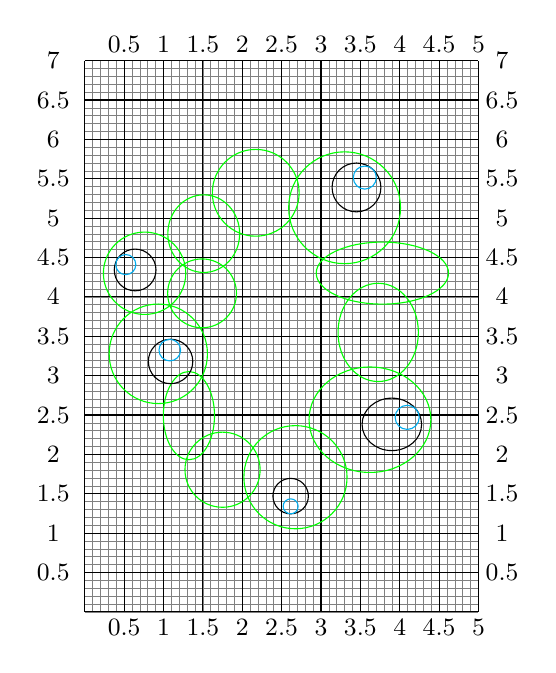
\begin{tikzpicture}
  %\draw node at (2.5,3.5) {\includegraphics[width=0.73\hsize]{./inc_op_b.png}};
  \draw [help lines, step=0.1cm] (0,0) grid (5,7);
  \draw [step=0.5cm] (0,0) grid (5,7);
  \foreach \x in {0.5,1,...,5} \node at (\x,-0.2) {\small\x} node at (\x,7.2) {\small\x};
  \foreach \x in {0.5,1,...,7} \node at (-0.4,\x) {\small\x} node at (5.3,\x) {\small\x};
  \draw [green] (2.676,1.71) circle [radius=0.655];
  \draw [black] (2.615,1.47) circle [radius=0.225];
  \draw [cyan] (2.615, 1.34) circle [radius=0.095];
  \draw[green] (1.75, 1.805) circle [radius=0.477];
  \draw[green] (1.323, 2.492) circle [x radius=0.325, y radius=0.56];
  \draw[green] (0.934, 3.277) circle [x radius=0.624, y radius=0.632];
  \draw[black] (1.09, 3.18) circle [radius=0.282];
  \draw [cyan] (1.08, 3.324) circle [radius=0.137];
  \draw[green] (0.76, 4.3) circle [radius=0.523];
  \draw[black] (0.64, 4.342) circle [radius=0.265];
  \draw [cyan] (0.521, 4.41) circle [radius=0.1275];
  \draw[green] (1.49, 4.045) circle [radius=0.437];
  \draw[green] (1.5112,4.803) circle [x radius=0.456, y radius=0.493];
  \draw[green] (2.1715, 5.322) circle [radius=0.551];
  \draw[green] (3.3,5.132) circle [radius=0.71];
  \draw[black] (3.451, 5.39) circle [radius=0.31];
  \draw[cyan] (3.557, 5.515) circle [radius=0.1463];
  \draw[green] (3.78, 4.302) circle [x radius=0.84, y radius=0.394];
  \draw[green] (3.727, 3.549) circle [x radius=0.51, y radius=0.624];
  \draw[green] (3.622, 2.44) circle [x radius=0.7735, y radius=0.6695];
  \draw[black] (3.9, 2.381) circle [x radius=0.378, y radius=0.333];
  \draw[cyan] (4.095, 2.47) circle [radius=0.153];
\end{tikzpicture}
\end{figure}
\end{document}
